
\procTitle{Разнообразие услуг в~жилой зоне, как фактор социально-экономического развития региона}

\procAuthor{Кодырев~Е.\,Д., Лунегова~А.\,А., Болотин~А.\,В.}
\procEmail{egor.k99@mail.ru, laaru@rambler.ru, alexandr\_bolotin@mail.ru}
\procOrganization{СВГУ}
\procCity{Магадан}


\makeProcTitle
\index{l@Лунегова~А.\,А.}
\index{b@Болотин~А.\,В.}
\index{k@Кодырев~Е.\,Д.}

Основной функцией региональных органов власти является социально-экономическое развитие региона. Социально-экономическое развитие региона~--- многомерный и~многоаспектный процесс, который состоит из~совокупности факторов, как экономических, так и~социальных. В период структурных преобразований в~социально-экономической системе вопросы дальнейшего экономического и~социального развития региона требуют дополнительного изучения, в~этом заключается актуальность исследования.

В управлении развитием региона власти применяют широкий спектр действий, направленных на стимулирование развития экономики в~целом. С помощью имеющихся и~вновь разрабатываемых механизмов управления создаются новые рабочие места, расширяются возможности для тех видов экономической деятельности, в~которых заинтересовано местное население.

Выявление факторов, влияющих на темпы социально-экономического развития региона, имеет важное значение. Одним из~таких факторов является формирование комфортной городской среды. Комфортная городская среда проживания в~настоящее время предопределяет экономические темпы развития региона в~целом, влияет на социально-политическую обстановку, темпы миграции населения и~привлечение инвестиций. Регионам, заинтересованным в~совершенствовании социально-экономического взаимодействия путём формирования комфортной городской среды, следует улучшать материальные и~нематериальные составляющие внутреннего факторного пространства.

Инструментом для оценки качества материальной городской среды и~ус\-ло\-вий её формирования, позволяющим использовать результаты оценки для создания рекомендаций по~улучшению среды, является индекс качества городской среды.

Индекс формируется Министерством строительства и жилищно-ком\-му\-наль\-но\-го хозяйства РФ. Результаты формирования Индекса используются в реализации положений Указа Президента Российской Федерации от 7 мая 2018~г. №~204 <<О национальных целях и стратегических задачах развития Российской Федерации на период до 2024 года>> [4], национального проекта <<Жилье и городская среда>> [3], в том числе для определения размера субсидии из~федерального бюджета бюджетам субъектов Российской Федерации на~поддержку государственных программ субъектов Российской Федерации и~муниципальных программ формирования современной городской среды.

Городская среда характеризуется совокупностью природных, ар\-хи\-тек\-тур\-но-пла\-ни\-ро\-воч\-ных, экологических и~других факторов, формирующих среду жизнедеятельности города на определённой территории и~определяющих комфортность проживания на этой территории. Индекс города представляет собой цифровое значение (в баллах) состояния городской среды, полученное в~результате комплексной оценки количественных и~поддающихся измерению индикаторов, характеризующих уровень комфорта проживания в~соответствующем городе.

На основе совокупности значений индикаторов определяются следующие уровни качества городской среды:
\begin{itemize}[noitemsep]\vspace{-8pt}
  \item благоприятная городская среда~--- состояние городской среды, при котором количество набранных баллов составляет более 50\,\% максимально возможного количества баллов индекса города;
  \item неблагоприятная городская среда~--- состояние городской среды, при котором количество набранных баллов составляет менее 50\,\% максимально возможного количества баллов индекса города [2].
\end{itemize}
 \vspace{-8pt}\enlargethispage{\baselineskip}
Формирование комфортной городской среды и~её влияние на социально-экономическое развитие региона рассмотрено на материалах г. Магадана. На рис. 1 представлен индекс и~его составляющие индикаторы качества городской среды г.~Магадана по~состоянию на конец 2019~г.

\begin{figure}[h!]
  \begin{center}
    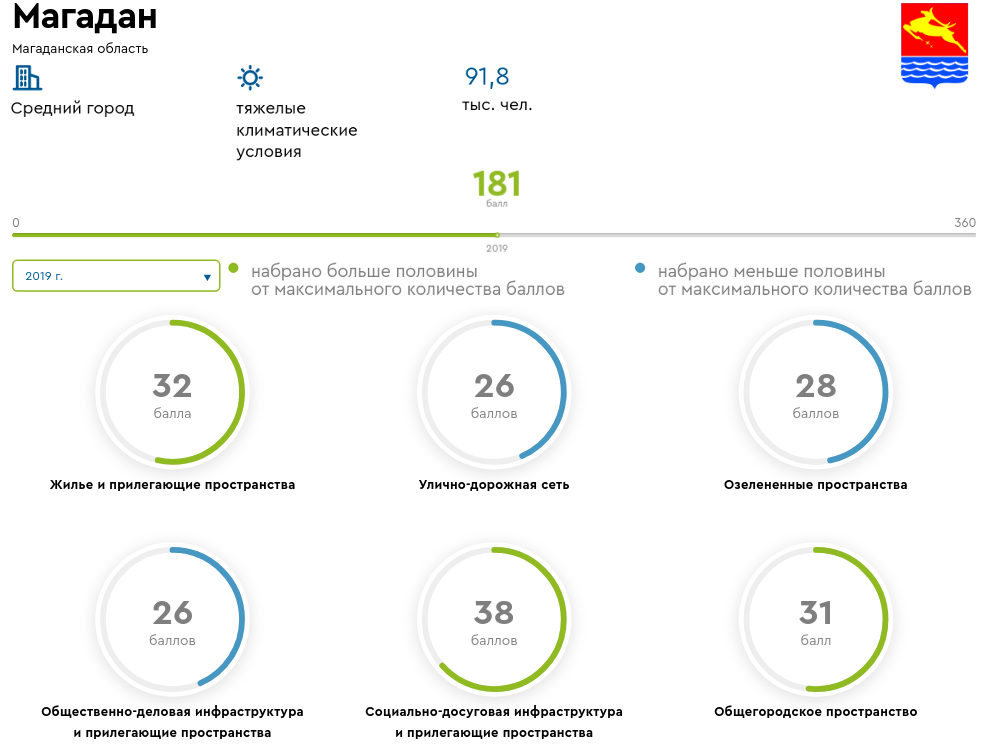
\includegraphics[width=1\textwidth]{authors/kodirev-fig-1.png}
  \end{center}
  \caption{Индекс и его составляющие индикаторы качества городской среды г.~Магадана за~2019~г.~[1]}
  \label{fig:kodirev-fig-1}
\end{figure}


Как видно из~рисунка 2, три из~шести показателей индекса качества
городской среды находятся в~зеленой, <<благоприятной>> зоне, т.\,е. данные показатели превышают пороговый уровень, равный тридцати баллам: жилье и~прилегающие пространства, социально-досуговая инфраструктура и
прилегающие пространства. Причем, каждая составляющая индекса качества
городской среды определяется из~шести индикаторов, характеризующих
данный показатель.

В качестве объекта исследования рассматривался микрорайон <<Автотек>> г.~Магадана, карта местности которого представлена на рис.~2. В исследовании проанализирован один из~показателей индекса
качества городской среды <<Общегородское пространство>> и~один из~его
индикаторов <<Разнообразие услуг в~жилой зоне>>, который характеризует
разнообразие жилой зоны исходя из~наличия в~ней объектов инфраструктуры
с функциями назначения, отличными от жилой зоны. Следует отметить, что
по итогам 2019~г. значение данного показателя составило 31~балл, что
дает нам основание для дальнейшего изучения данного вопроса с~целью
развития общегородского пространства.


\begin{figure}[h!]
  \begin{center}
    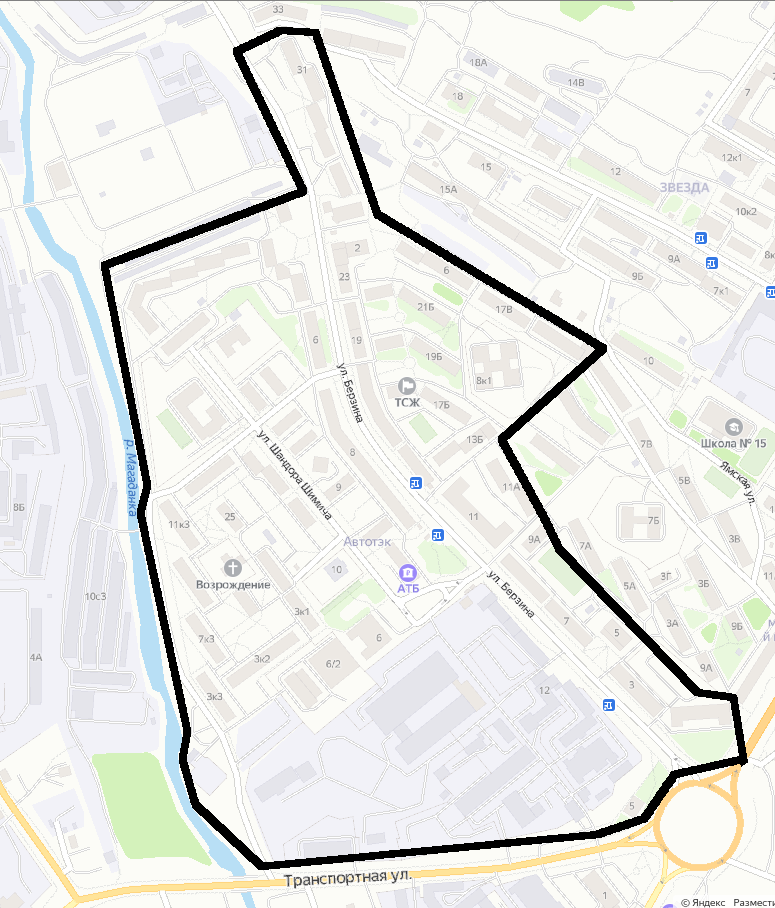
\includegraphics[width=0.8\textwidth]{authors/kodirev-fig-2.png}
  \end{center}
  \caption{Карта местности микрорайона <<Автотэк>> по состоянию на 01.03.2020~г.}
  \label{fig:kodirev-fig-2}
\end{figure}


Микрорайон насчитывает 51~дом, которые расположены по~улицам: Шандора Шимича, Берзина, Левонабережная, Ямская, Колымская. В табл.~1 представлены организации и~предприятия, размещенные в~зоне жилой застройки.

\begin{table}[h!]
\caption*{\textbf{Организации и предприятия, размещенные в микрорайоне <<Автотек>> по состоянию на 01.03.2020 г.}}
\label{tab:kodirev-tab-1}
\begin{changemargin}{-1cm}{-1cm}
\begin{tabular}{p{5cm}p{7cm}cc}
   \toprule
Назначение предприятия, организации &
Наименование предприятия, организации &
 \parbox[c][][c]{0.1\textwidth}{ \centeringКол-во, ед.} &
  \parbox[c][][c]{0.1\textwidth}{ \centeringУд. вес, \%} \\
   \toprule
Учреждение 				образования              & Муниципальное 				бюджетное дошкольное образовательное 				учреждение Центр развития ребенка 				Детский сад №~63 <<Дельфиненок>>                            & 1               & 2,8               \\
                                        & Магаданский 				лицей индустрии питания и сферы услуг 				№5                                                                                              & 1               & 2,8               \\
                                        & Муниципальное 				автономное общеобразовательное 				учреждение Средняя общеобразовательная 				школа с углубленным изучением отдельных 				предметов №~4 & 1               & 2,8               \\ \midrule
Учреждение 				здравоохранения          & Детская 				поликлиника №~2                                                                                                                               & 1               & 2,8               \\ \midrule
Учреждение 				культуры                 & Муниципальное 				бюджетное учреждение культуры города 				Магадана Молодежный культурный центр                                                           & 1               & 2,8               \\ \midrule
Учреждение 				таможенного контроля     & Магаданская 				таможня, отдел таможенного оформления 				и таможенного контроля                                                                          & 1               & 2,8               \\ \midrule
Учреждение 				страхования              & Территориальный 				фонд обязательного медицинского 				страхования <<СОГАЗ Мед>>                                                                           & 1               & 2,8               \\ \midrule
Некоммерческие 				организации          & Протестантская 				церковь Христианская миссионерская 				церковь Возрождения                                                                             & 1               & 2,8               \\
                                        & Товарищество 				собственников жилья                                                                                                                      & 2               & 5               \\ \midrule
Банк                                    & Банк 				<<Азиатско-Тихоокеанский банк>>                                                                                                                    & 1               & 2,8               \\ \midrule
Библиотека                              & Магаданская 				областная юношеская библиотека                                                                                                            & 1               & 2,8               \\ \midrule
Услуги 				населению                    & Кабельное 				телевидение <<Мир антенн>>                                                                                                                    & 1               & 2,8               \\
                                        & Парикмахерская 				<<Шадэ Style>>                                                                                                                           & 1               & 2,8               \\
                                        & Транспортная 				компания <<Вилкон>>                                                                                                                        & 1               & 2,8               \\ \midrule
Предприятия 				общественного питания   &  кафе <<Кавказ>>                                                                                                                     & 1               & 4               \\ \midrule
Предприятия 				розничной торговли      & Продуктовый, 				промтоварный, овощной, хлебный, 				алкоголь, цветы, золото и т.\,п.                                                                       & 19              & 54,9              \\  \bottomrule
                                        & Всего учреждений и предприятий                                                                                                                            & 35              & 100\\


                                        \bottomrule
\end{tabular}
\end{changemargin}
\end{table}


На территории микрорайона <<Автотек>> размещены 35 предприятий и~организаций различных форм собственности и~организационно-правовых форм. Среди них половина принадлежит предприятиям розничной торговли. Исследование выявило, что принципы размещения розничных торговых предприятий в~городах в~данном микрорайоне соблюдены. Розничная торговая сеть максимально приближена к~населению. Радиус их деятельности составляет примерно 500~м. Из этого следует, что одно из~основных требований культуры торговли <<удобство для населения>> достигнуто, так как:
\begin{enumerate}[noitemsep]\vspace{-8pt}
  \item магазины максимально приближены к~потребителю;
  \item в~них обеспечена возможность приобретения товаров сложного ассортимента жителями ближайшего микрорайона;
  \item равномерно, пропорционально численности населения, размещены однотипные магазины;
  \item комплексно расположены магазины с~ассортиментом товаров, связанных общностью спроса;
  \item обеспечены условия рентабельной работы для каждого торгового предприятия.
\end{enumerate}
 \vspace{-8pt}

На рис.~3 представлены положительные социальные и~экономические составляющие, являющиеся следствием размещения в~зоне застройки <<Автотек>> предприятий различного назначения.

\begin{figure}[H]
  \centering
  \includegraphics[width=1\textwidth, page=1]{authors/kodirev-fig-3.pdf}
  \caption{Социально-экономический эффект разнообразия услуг в~зоне жилой застройки}
  \label{fig:kodirev-fig-3}
\end{figure}

К социальным факторам относят потребность в~снижении затрат времени населения на посещение предприятий торговли, необходимость повышения уровня его обслуживания. К~экономическим факторам размещения предприятий розничной торговли относятся: обеспечение оптимального уровня доходности розничной торговой сети, возмещение затрат на строительство и~эксплуатацию розничной торговой сети.

Общая жилая площадь микрорайона <<Автотек>> равна 126,9~тыс.~м$^2$, площадь не жилых функциональных участков~--- 92,8~тыс.~м$^2$.

Разнообразие услуг в~жилой зоне:

$$ P_{\text{усл.}} = \frac{S_{\text{уфс.}}}{S_{\text{жил.}}}\cdot100 = \frac{92,8}{126,9} = 73,2\,\%,$$

где $P_{\text{усл.}}$~--- показатель индикатора <<Разнообразие услуг в~жилой зоне>>;
$S_{\text{уфс.}}$~--- площадь не жилых функциональных участков, м$^2$;
$S_{\text{жил.}}$~--- общая жилая площадь микрорайона <<Автотек>>, м$^2$.

Индикатор, комплексно характеризует разнообразие возможностей в~микрорайоне. Высокая доля третичного сектора экономики в~микрорайоне говорит о большом разнообразии видов деятельности и~работ и~большом количестве организаций, которые позитивно влияют на социально-экономические параметры микрорайона и~городской среды. Такой подход социально-экономического развития страны, выбранный Правительством РФ, позволяет развить даже в~самых отстающих регионах и~небольших муниципальных образованиях как основные отрасли народного хозяйства~--- строительство, промышленность, сельское хозяйство, транспорт, так и~непроизводственную сферу экономики.

Исследование выявило, что принципы размещения розничных торговых предприятий в~данном микрорайоне соблюдены. Розничная торговая сеть максимально приближена к~населению. Радиус их деятельности составляет примерно 500~м. Из этого следует, что одно из~основных требований культуры торговли «удобство для населения» достигнуто, так как:
\begin{itemize}[noitemsep]\vspace{-8pt}
\item магазины максимально приближены к~потребителю;
\item в~них обеспечена возможность приобретения товаров сложного ассортимента жителями ближайшего микрорайона;
\item равномерно, пропорционально численности населения, размещены однотипные магазины;
\item комплексно расположены магазины с~ассортиментом товаров, связанных общностью спроса;
\item обеспечены условия рентабельной работы для каждого торгового предприятия.
\end{itemize}\vspace{-8pt}

Таким образом, обустройство пространства микрорайона <<Автотек>> выявило высокую степень разнообразия услуг в~жилой зоне. При этом, чем большая площадь жилой зоны признается разнообразной, тем активней в~данной зоне протекают социально-экономические процессы, что в~свою очередь способствует повышению экономических темпов развития региона в~целом.


\begin{thebibliography}{99}
\bibitem{}Индекс качества городской среды Магадана.~--- 2018.~--- URL:~https://индекс-городов.рф/\#/cities/2012 (Дата обращения: 20.03.2020).
\bibitem{}Об утверждении методики формирования индекса качества городской среды. Распоряжение Правительства Российской Федерации от 23~марта 2019~года №~510-р (с изменениями на 5~ноября 2019 года) // Docs.cntd.ru, все Кодексы РФ, СП, ГОСТ, Снип, Санпин, регламенты, указы, законы.~--- URL: http://docs.cntd.ru/document/553937399 (Дата обращения: 10.03.2020).
\bibitem{}Национальный проект <<Жилье и~городская среда>> // Минстрой России.~--- Системные требования: Adobe Acrobat Reader.~--- URL: https://minstroyrf.gov.ru/upload/iblock/426/Pasport-natsionalnogo-proekta-\_ZHile-i-gorodskaya-sreda\_.pdf (Дата обращения: 10.03.2020).
\bibitem{}Указ Президента Российской Федерации от 7~мая 2018~г. №~204 <<О национальных целях и~стратегических задачах развития Российской Федерации на период до 2024 года>> // Президент России.~--- URL: http://www.kremlin.ru/acts/bank/43027 (Дата обращения: 20.03.2020).

\end{thebibliography}
